% ------------------------------------------------------------------
\documentclass[12 pt]{article} % A4 paper set by geometry package below
\pagenumbering{arabic}
\setlength{\parindent}{10 mm}
\setlength{\parskip}{12 pt}

% Nimbus Sans font should be reasonably legible
\usepackage{helvet}
\renewcommand{\familydefault}{\sfdefault}
\usepackage[T1]{fontenc}  % Without this \textsterling produces $

% Section header spacing
\usepackage{titlesec}
\titlespacing\section{0pt}{12pt plus 4pt minus 2pt}{0pt plus 2pt minus 2pt}
\titlespacing\subsection{0pt}{12pt plus 4pt minus 2pt}{0pt plus 2pt minus 2pt}
\titlespacing\subsubsection{0pt}{12pt plus 4pt minus 2pt}{0pt plus 2pt minus 2pt}

\usepackage{amsmath}
\usepackage{amssymb}
\usepackage{graphicx}
\usepackage{verbatim}    % For comment
\usepackage[paper=a4paper, marginparwidth=0 cm, marginparsep=0 cm, top=2.5 cm, bottom=2.5 cm, left=3 cm, right=3 cm, includemp]{geometry}
\usepackage[pdftex, pdfstartview={FitH}, pdfnewwindow=true, colorlinks=true, citecolor=blue, filecolor=blue, linkcolor=blue, urlcolor=blue, pdfpagemode=UseNone]{hyperref}

% Put module code and last-modified date in footer
\usepackage{fancyhdr}
\pagestyle{fancy}
\fancyhf{}
\renewcommand{\headrulewidth}{0pt}
\cfoot{{\small \thisweek}\hfill \thepage\hfill {\small \moddate}}

% Hopefully address Canvas complaints about pdf tagging
%\usepackage[tagged]{accessibility}
\hypersetup {
  pdfauthor={David Schaich},
  pdftitle={Statistical Physics Tutorial Problem},
}
% ------------------------------------------------------------------



% ------------------------------------------------------------------
% Shortcuts
\newcommand{\la}{\ensuremath{\lambda} }
\newcommand{\lath}{\ensuremath{\la_{\mathrm{th}}} }
\newcommand{\Om}{\ensuremath{\Omega} }
% ------------------------------------------------------------------



% ------------------------------------------------------------------
\begin{document}
\newcommand{\thisweek}{MATH327 Tutorial (Cycle)}
\newcommand{\moddate}{Last modified 11 Mar.~2022}
\begin{center}
  {\Large \textbf{MATH327: Statistical Physics, Spring 2022}} \\[12 pt]
  {\Large \textbf{Tutorial problem \ --- \ Otto cycle}} \\[24 pt]
\end{center}

The figure below shows the `Otto cycle' that describes an idealized petrol engine.
The compression and expansion (`power') stages are adiabatic, while the volume is fixed at $V_2$ for the `ignition' stage that burns the fuel to produce heat, and at $V_1 > V_2$ for the `exhaust' stage that replaces the burnt fuel with cooler, fresh gas.
The \textbf{compression ratio} is defined as $r \equiv V_1 / V_2 > 1$.

\begin{center}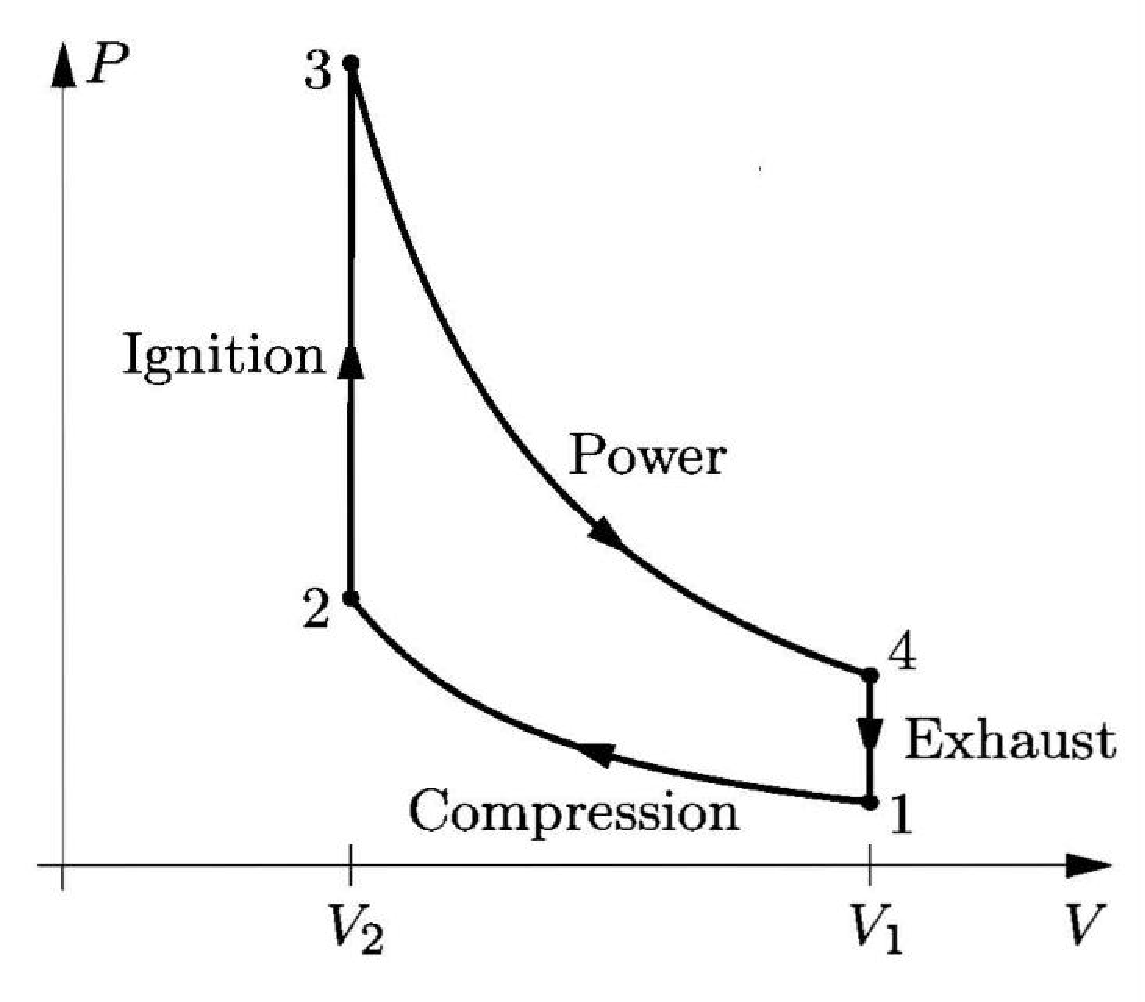
\includegraphics[width=0.8\textwidth]{figs/Otto.pdf}\end{center}

The efficiency $\eta$ of the Otto cycle depends \emph{only} on the compression ratio $r$.
What is this efficiency?
How does it compare to the efficiency of the Carnot cycle?
How should $V_1$ and $V_2$ be chosen to maximize the efficiency?

\textbf{Hint:} Given the labels in the diagram above, $T_1$ would be the low temperature of the cold reservoir while $T_3$ would be the high temperature of the hot reservoir.
The corresponding Carnot cycle efficiency is therefore $\eta_{\text{Carnot}} = 1 - \frac{T_1}{T_3}$, and the comparison is easiest if the Otto cycle efficiency is expressed in terms of temperatures rather than volumes.

\end{document}
% ------------------------------------------------------------------
